\begin{section}{System Models and Architecture}
	
\label{sec:modeling}
In this section, the system dynamical, noise, and disturbance models used for control and motion are described, as well as the adaptive control scheme and confidence interval model.

% Bold letters only for vectors
% Approach

\subsection{Vehicle Model}
To attain a dynamical model of the ground vehicle, a generalized differential-drive model may be used (CITE). The vehicle's position is described by its $x$ and $y$ coordinates, $\theta$ represents the vehicle's heading angle measured from the $x$ axis, and $v$ is the speed in the direction in this direction. $F_l$ and $F_r$ describe the left and right forces from the wheels, while $B_r$ is the mechanical resistance of the wheels to rolling. If the assumption is that the wheels do not slip, the continuous time dynamical model of the vehicle is
    \begin{align}
        \dot{v}=\begin{cases}
            \frac{1}{m}(F_l+F_r-(B_s+B_r)v), & \text{if turning},\\
            \frac{1}{m}(F_l+F_r-B_rv), & \text{if not turning},
        \end{cases}\\
        \dot{\omega}=\begin{cases}
            \frac{1}{I_z}(\frac{B}{2}(F_l-F_r)-B_l\omega), &\text{if turning},\\
            0, & \text{if not turning},
        \end{cases}
	\end{align}
	\begin{align}
        \dot{\theta}=\omega, \dot{x}=v\sin(\theta), \dot{y}=v\cos(\theta).
	\end{align}
This presents a high-level model of the vehicle, describing only the motion equations. Both forces, $F_l$ and $F_r$, are considered as inputs to the system, are derived from the vehicle's electromotors and are affected by the motors, gearbox, and wheels. The above continuous-time dynamical equations will be discretized into a form that's suitable for the discrete time adaptive controller.

 \subsection{Noise and Disturbance Model}
When a ground vehicle is in motion, there are many factors that may cause it to behave differently. These factors can include sensor or actuator noises and actuator failure, as well as external influences like wind disturbance, and a changing ground surface. The uncertainties from actuator noise are due to mechanical uncertainties of motors and gears, which are represented by $ \eta_a \in N(0,\sigma_a) $. The uncertainty due to measurement noise of the sensors is described by $ \eta_s \in N(0,\sigma_s) $. All noises are assumed to have a zero mean Gaussian distribution.


\subsection{Adaptive Control Model}
The control algorithm used is characteristic polynomial adaptive control based on the following discrete-time state space model with known dimensions of $A$ and $B$:
	\begin{equation}
	\bm{x}(k+1) = \bm{A}\bm{x}(k) + \bm{B}\bm{u}(k)
	\end{equation}
with its discrete time transfer function:
	\begin{align}
        & G(z) = \frac{y(z)}{u(z)} = \bm{C}(z\bm{I}-\bm{A})^{-1}\bm{B} \nonumber \\ 
	& = \frac{b_0z^{n-d}+b_1z^{n-d-1} +...+b_mz^{n-d-m}}{z^{n}+a_1z^{n-1}+...+a_{n-1}z+a_n}
	\end{align}
where $b_0\ne{0}$, $d>0$, and $n-d-m\geq{0}$\\
Using an ARMA model and defining the operators $q^{-1}$ (delay) and q (advance),
	\begin{equation}
	q^{-1}x(k) = x(k-1), qx(k) = x(k+1)
	\end{equation}
the system is now expressed as:
	\begin{align}
	& (1+a_1q^{-1}+...+a_nq^{-n})y(k) \nonumber \\
	& =q^{-d}(b_0+b_1q^{-1}+...+b_mq^{-m})u(k)
	\end{align}
where:
	\begin{equation}
	Aq^{-1}y(k)=q^{-d}B^{'}(q^{-1})u(k)
	\end{equation}
The objective of model reference adaptive control is to calculate an input signal u(k) such that the system tracks the signal $y^{*}(k)$ given the reference signal r(k). The reference model the system is trying to follow is expressed as:
	\begin{equation}
	E(q^{-1})y^*(k+d)=q^{-d}gH(q^{-1})r(k)
	\end{equation}
This system is parametrized as:
	\begin{equation}
	E(q^{-1})y(k+d)={\alpha}q^{-1}y(k) + {\beta}q^{-1}u(k)=\theta_0^T\phi(k)
	\end{equation}
	\begin{equation}
	\alpha(q^{-1})=G(q^{-1})=\alpha_0+\alpha_1q^{-1}+ \dots +\alpha_{n-1}q^{-n+1}
	\end{equation}
	\begin{align}
	\beta( & q^{-1})=F(q^{-1})B^{'}(q^{-1})=\beta_0+\beta_1q^{-1} \nonumber \\
	& + \dots +\beta_{m+d-1}q^{-m-d+1}, \beta_0\neq0
	\end{align}
	\begin{equation}
	E(q^{-1})=F(q^{-1})A(q^{-1})+q^{-d}G(q^{-1})
	\end{equation}
	Assumptions for adaptive control: 
	\begin{enumerate}
	\item all zeros of $B^{'}(z^{-1})z^m$ are within $|z|<1$. 
	\item $n$ and $m$ (or their upper bounds) are known. 
	\item the system delay $d$ is known.
	\end{enumerate}
Parametrization to express this system is:
	\begin{equation}
	\theta_0=(\alpha_0, \dots ,\alpha_{n-1},\beta_0, \dots ,\beta_{m+d-1})^T \in R^{n+m+d}
	\end{equation}
	\begin{align}
	& \phi(j)=(y(k), \dots ,y(k-n+1),u(k), \dots , \nonumber \\
	& u(k-m-d+1))^T \in R^{n+m+d}
	\end{align}
where $\theta_0$ is unknown and $\phi(k)$ is known.
	The adaptive control input u(k) is then calculated from the equation:
	\begin{equation}
	\theta^T(k)\phi(k)=E(q^{-1})y^{*}(k+d)
	\end{equation}
with the equation for the input u(k) as:
	\begin{align}
	& u(k)=\frac{1}{\theta_{n+1}(k)}(-\theta_1(k)y(k)-\theta_2(k)y(k-1)- \dots  \nonumber \\
	& -\theta_n(k)y(k-n-1)-\theta_{n+2}(k)u(k-1) \nonumber \\
	& -\theta_{n+3}(k)u(k-2)- \dots - \theta_{n+m+d}(k)u(k-m-d+1) \nonumber \\
	& +y^{*}(k+d))^T
	\end{align}
	\begin{equation}
	\theta(k)=(\theta_1(k), \dots ,\theta_n(k),\theta_{n+1}(k), \dots ,\theta_{n+m+d}(k))^T
	\end{equation}
where $\theta(k)$ is the estimate of the true parameter vector $\theta_0$, updated by:
	\begin{equation}
	\theta(k)=\theta(k-1)+\frac{a(k)\phi(k-d)e(k)}{c+\phi^T(k-d)\phi(k-d)}
	\end{equation}
	\begin{equation}
	e(k)=E(q^{-1})y(k)-\theta^T(k-1)\phi(k-d)
	\end{equation}
	\begin{align*}
	\varepsilon<a(k)<2-\varepsilon, 0,\varepsilon<1, c>0
	\end{align*}
To avoid division by 0, $\theta_{n+1}(k)\neq0$ is necessary.


 \subsection{Confidence Intervals}

Confidence intervals are used to estimate the mean of a population of data in stochastic environments. Using this method, a guarantee can be made that the mean of the data has a specific percentage of confidence that it's within an interval. Assuming the knowledge of the confidence percentage $ \bm{z^{*}} $, sensor noise population standard deviation $ \bm{\sigma_p} $, the number of sensor data samples $ \bm{N} $, and the mean of the data samples $ \bm{\bar{x}}_{x,y} $ in the $\bm{x}$ and $\bm{y}$ direction, a confidence interval of a certain percentage can be calculated: 
 	\begin{equation}
		CI_{x,y|N} = \bar{s}_{x,y} + z^{*}\frac{\sigma}{\sqrt{N}}
	\end{equation}
This is under the assumption that the mean is not changing over the previous $\bm{N}$ number of sampled data points used in the current confidence interval calculation. A detailed approach to we compensate for a translating system will be shown in (REF THE SECTION HERE).

%NEED TO INCLUDE EQUATION TO SHOW HOW WE ESTIMATED A STATIC CASE BY TRANSLATING THE PAST DATA POINTS RIGHT HERE!

%\begin{figure*}
%\centering
%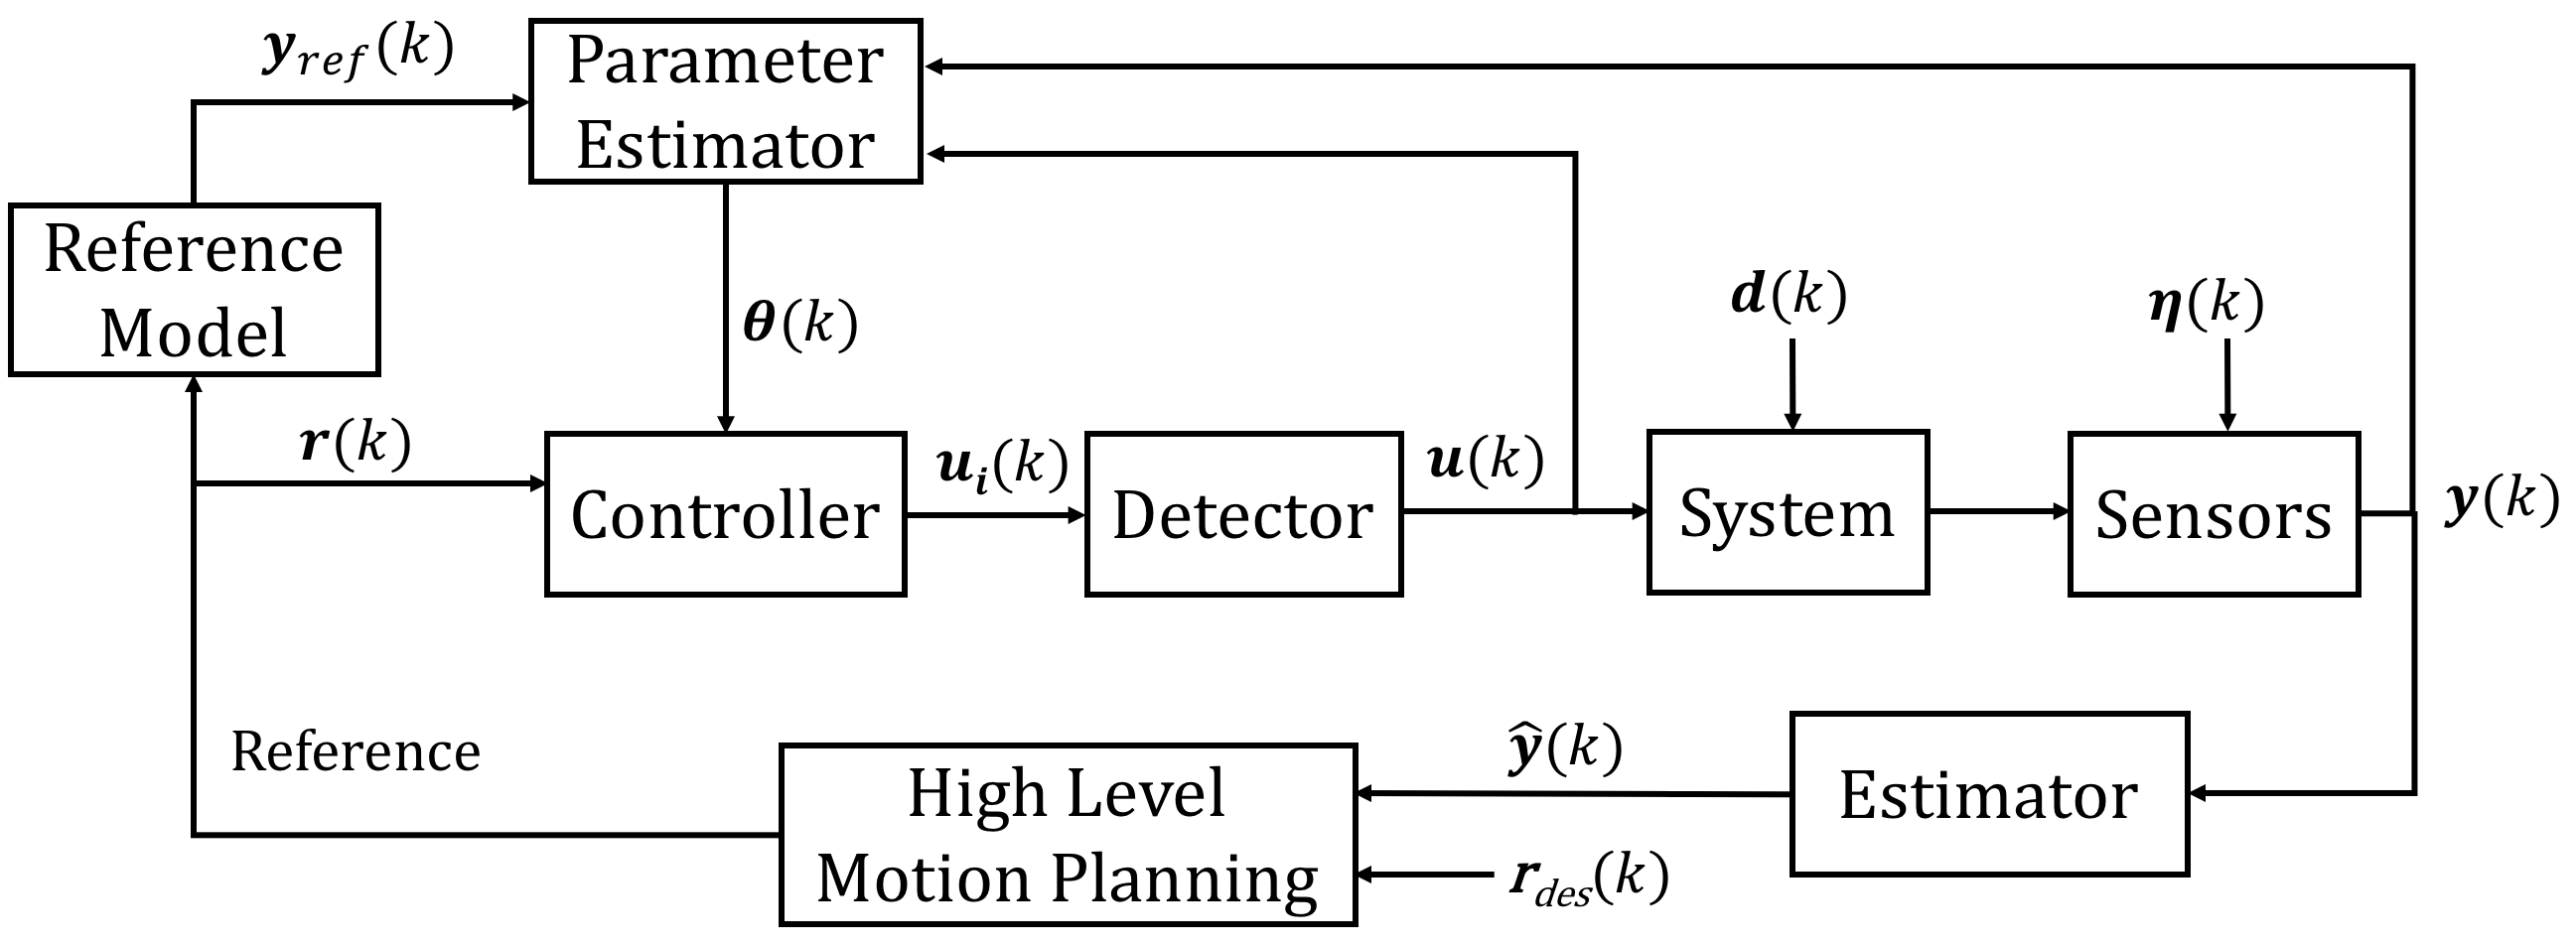
\includegraphics[width = 0.9\textwidth]{sys_arch.png}
%\caption{Overall system architecture showing the relationship between the reference model adaptive controller and the adaptive motion planner.}
%\label{fig:system_arch}
%\end{figure*}

\begin{figure}
\vspace{1pt}
\centering
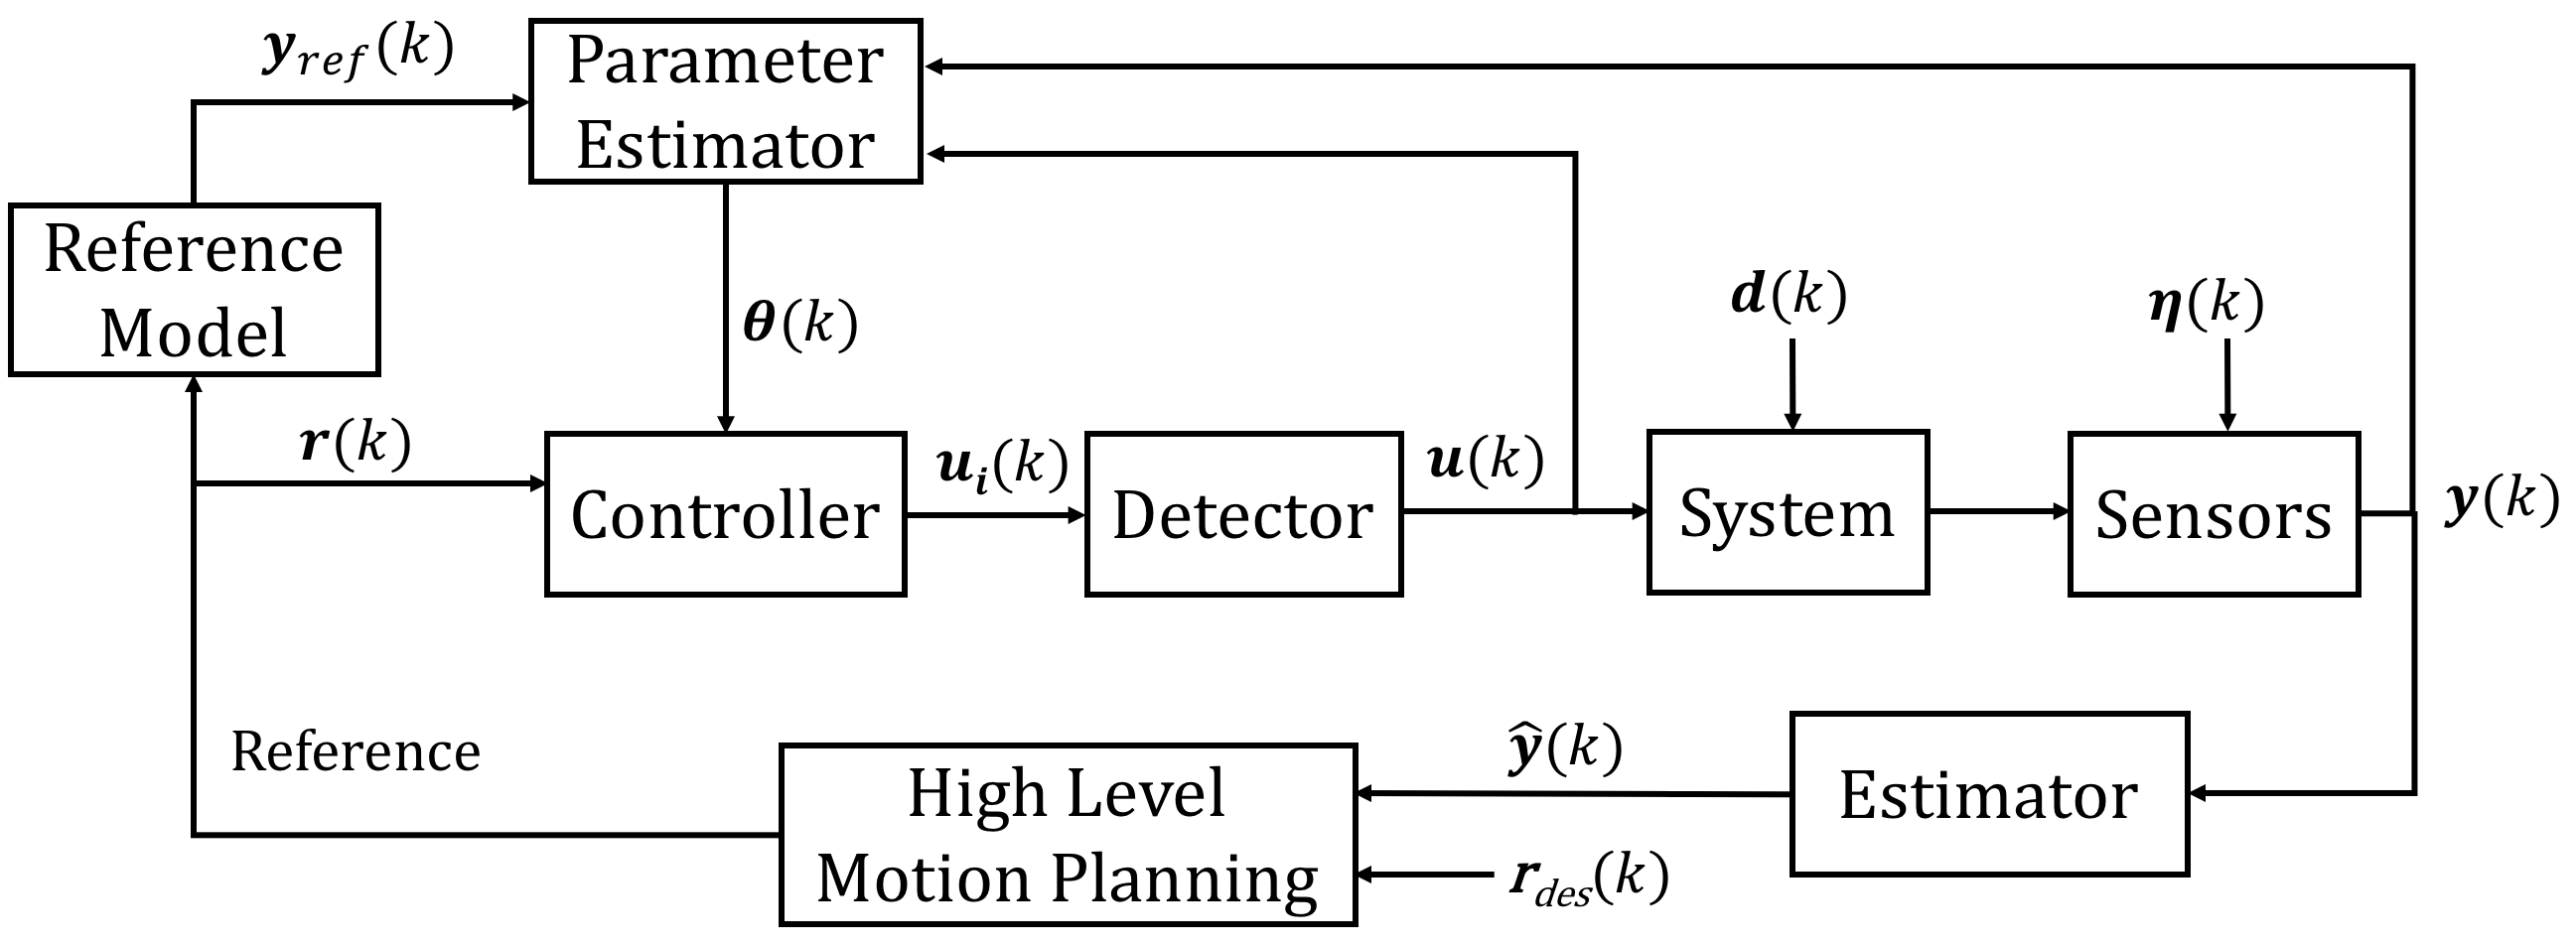
\includegraphics[width=0.48\textwidth]{sys_arch.png}
\caption{Overall system architecture showing the relationship between the reference model adaptive controller and the adaptive motion planner.}
\label{fig:system_arch}
\end{figure}



\end{section}